\documentclass[openright,twoside,10pt]{book}
\usepackage[b5paper,left=2cm,top=2.5cm,right=1.5cm,bottom=2.5cm]{geometry} 
\usepackage[spanish]{babel} % espanol
\usepackage[utf8]{inputenc} % acentos sin codigo
\usepackage{graphicx} % gráficos
\usepackage{lscape}
\usepackage{fancyvrb}
\usepackage{fancyhdr}
\usepackage{wrapfig}
\usepackage{hyperref}
\usepackage{biblatex}
\usepackage{float}

\providecommand{\tightlist}{%
  \setlength{\itemsep}{0pt}\setlength{\parskip}{0pt}}
  
\setlength{\parskip}{10pt plus 1pt minus 1pt}
 % aqui definimos el encabezado de las paginas pares e impares.
\rhead[]{}

\renewcommand{\headrulewidth}{0.5pt}

% aqui definimos el pie de pagina de las paginas pares e impares.
\rfoot[\thepage]{\thepage}
\cfoot[]{}
\renewcommand{\footrulewidth}{0pt}

%redefino el verbatim
%\renewenvironment{verbatim}{\begin{Verbatim}[frame=single,fontsize=\small]}{\end{Verbatim}}


% aqui definimos el encabezado y pie de pagina de la pagina inicial de un capitulo.
\fancypagestyle{plain}{
\fancyhead[R]{}
\fancyfoot[C]{}
\fancyfoot[R]{\thepage}
\renewcommand{\headrulewidth}{0.5pt}
\renewcommand{\footrulewidth}{0pt}
}

\pagestyle{fancy} % seleccionamos un estilo





\date{22 de junio de 2017}
\author{Julio Gracia Gutiérrez}
\title{Desarrollo de software educativo de apoyo a la docencia en la teoría de
grafos.}

\begin{document}
    \begin{titlepage}
        \begin{center}
            \vspace*{-1in}
            \begin{figure}[htb]
                \begin{center}
                    
\includegraphics[width=3cm]{./latex/img/logo}
                \end{center}
            \end{figure}
            \begin{large}
                \textbf{Universidad de Valladolid}
            \end{large}

            \vspace*{0.15in}
            \vspace*{0.6in}
            \begin{large}
                \textbf{ESCUELA DE INGENIERÍA INFORMÁTICA}
            \end{large}
            \vspace*{0.2in}
            \textbf{ GRADO EN INGENIERÍA INFORMÁTICA}\\
            \textbf{ MENCIÓN EN INGENIERÍA DE SOFTWARE }
            \vspace*{0.5in}
            \rule{140mm}{0.1mm}\\
            \vspace*{0.3in}
            \begin{large}
                \textbf{{\LARGE Desarrollo de software educativo de apoyo a la docencia en la teoría de
grafos.\\}}
            \end{large}
            \vspace*{0.6in}
            \rule{140mm}{0.1mm}\\
            \vspace*{2in}
            \begin{large}
                \begin{flushright}
                    \textbf{Alumno/a: Julio Gracia Gutiérrez \\
                    \vspace*{0.3in}
                    Tutores/as: María Felisa Pérez Martínez}
                \end{flushright}
            \end{large}
        \end{center}
    \end{titlepage}

    \newpage
    \mbox{}	
    \thispagestyle{empty} % para que no se numere esta página

    \chapter*{}
    \pagenumbering{Roman} % para comenzar la numeración de paginas en números romanos

    \begin{flushright}
        \textit{%Dedicatoria,\\
        Dedicatoria ejemplo}
    \end{flushright}

    \chapter*{Agradecimientos} % si no queremos que añada la palabra "Capitulo"
    \addcontentsline{toc}{chapter}{Agradecimientos} % si queremos que aparezca en el índice
    \markboth{AGRADECIMIENTOS}{AGRADECIMIENTOS} % encabezado 

    Agradecimiento ejemplo

    \chapter*{Resumen} % si no queremos que añada la palabra "Capitulo"
    \addcontentsline{toc}{chapter}{Resumen} % si queremos que aparezca en el índice
    \markboth{RESUMEN}{RESUMEN} % encabezado
    \begin{flushleft}

    En el presente trabajo se va a desarrollar un software de ayuda para la
    asignatura ``Matemáticas Discretas''. Se pretende que el alumno sea
    capaz de desarrollar un prototipo funcional de una aplicación web
    orientada a mejorar el aprendizaje y el afianzamiento de los conceptos
    relativos a la asignatura. En este punto es necesario plantear la
    arquitectura de la aplicación que vamos a implementar.
    
    La solución escogida consiste en utilizar Angular programado en
    TypeScript para el front-end, Node.js programado en JavaScript y una
    base de datos relacional MariaDB para el back-end. Angular es una
    plataforma de desarrollo para aplicaciones web de TypeScript de código
    abierto. Node.js es un entorno en tiempo de ejecución multiplataforma
    asíncrono, de código abierto, para la capa del servidor. MariaDB es un
    sistema de gestión de bases de datos derivado de MySQL.
    
    Palabras clave: Angular, Node.js, MariaDB, código abierto, TypeScript,
    JavaScript.

    \end{flushleft}


    \chapter*{Abstract} % si no queremos que añada la palabra "Capitulo"
    \addcontentsline{toc}{chapter}{Abstract} % si queremos que aparezca en el índice
    \markboth{ABSTRACT}{ABSTRACT} % encabezado
    \begin{flushleft}

    Traducción

    \end{flushleft}

    \tableofcontents % indice de contenidos

    \cleardoublepage
    \addcontentsline{toc}{chapter}{Lista de figuras} % para que aparezca en el indice de contenidos
    \listoffigures % indice de figuras

    \cleardoublepage
    \addcontentsline{toc}{chapter}{Lista de tablas} % para que aparezca en el indice de contenidos
    \listoftables % indice de tablas

    \chapter{Introducción}\label{introducciuxf3n}
    
    \section{Descripción del problema}\label{descripciuxf3n-del-problema}
    
    \pagenumbering{arabic}
    
    Los alumnos que entran en el primer curso de una ingeniería experimentan
    una grandes cambios a nivel académico. Esto es debido tanto a que cambia
    la metodología en la docencia, como al aumento del volumen de contenidos
    tanto teóricos como prácticos en comparación etapas anteriores. Algunas
    asignaturas se fundamentan en los conocimientos adquiridos durante los
    cursos de bachillerato pero otras tienen contenidos totalmente nuevos.
    La procedencia de los estudiantes es heterogénea: Bachillerato y PAU y
    Módulos Superiores y ,por tanto, habrán tenido diferente grado de
    contacto con los contenidos de la carrera. En particular, una de las
    asignaturas que no parten de contenido de cursos anteriores es
    Matemáticas Discretas, que incluye conceptos y relaciones matemáticas
    que no han sido explorados con anterioridad. Esta asignatura forma parte
    de las asignaturas del módulo básico (y común) de los Grados en
    Ingeniería.
    
    Con ella, se pretende ofrecer una formación básica y sólida al futuro
    ingeniero. Básica, en el sentido que los diferentes aspectos serán
    tratados a un nivel introductorio, y sólida, en el sentido de que los
    conocimientos adquiridos deben sentar las bases para desenvolverse en el
    resto de su formación académica y desarrollo profesional. Se trata de
    habilitar a los estudiantes para que adquieran las destrezas necesarias
    para seguir aprendiendo a lo largo de la vida los aspectos de la
    Informática relacionados con la lógica, teoría de conjuntos y
    combinatoria, como son la inteligencia artificial, el uso de bases de
    datos o la estadística.
    
    Teniendo en cuenta que la carga de esta asignatura es mayoritariamente
    teórica, el presente trabajo se va a centrar en mejorar el aprendizaje y
    la resolución de dudas respecto a la asignatura.
    
    Para tener una buena base en informática es necesario conseguir un buena
    base matemática teórica. En el primer año de carrera, los estudiantes
    pueden experimentar una falta de motivación en asignaturas de este tipo
    debido a la complejidad de las mismas y a que no consiguen encontrar una
    aplicación práctica real ni son conscientes de su importancia, tanto
    para asignaturas futuras como para su vida profesional.
    
    \section{Objetivo}\label{objetivo}
    
    El objetivo final de este trabajo es mejorar el estudio de la
    asignatura, facilitando el afianzamiento de los conocimientos. Para
    ello, se busca crear una plataforma que facilite la comunicación
    alumno-profesor, y dote al profesor de las herramientas para facilitar
    la distribución de los contenidos de la asignatura, así como permitiendo
    al alumno comprobar sus conocimientos mediante la implementación de
    tests. En definitiva, se busca mejorar el porcentaje de aprobados de la
    asignatura, ya que esta sienta unas bases muy importantes para otras
    asignaturas de cursos futuros.
    
    \section{Estructura de la memoria}\label{estructura-de-la-memoria}
    
    En base al esquema seguido para la realización del presente trabajo, se
    ha estructurado la memoria de la misma manera:
    
    PUNTO DE PARTIDA: En primer lugar se ha realizado un análisis del método
    educativo utilizado hasta el momento en la asignatura Matemáticas
    Discretas. Se ha revisado la guía docente de la asignatura con el fin de
    conocer los conocimientos teóricos y prácticos que, se pretende, el
    alumno adquiera.
    
    SOLUCIÓN ADOPTADA: Tras realizar el estudio del temario de la
    asignatura, se obtiene una solución que ayude a incentivar al alumno y
    le facilite el aprendizaje
    
    DESARROLLO DEL PROYECTO: La parte fundamental del proyecto es el
    desarrollo de un prototipo de plataforma web. En este apartado se
    profundizará en el proceso de desarrollo, que incluye las etapas de
    análisis, desarrollo y despliegue.
    
    CONCLUSIONES Y RESULTADOS: Tras realizar una serie de pruebas al
    prototipo, se presentarán las conclusiones y se analizarán los
    resultados así como posibles mejoras a tener en cuenta.
    
    \chapter{Punto de partida}\label{punto-de-partida}
    
    La metodología docente actual de la asignatura se basa en la combinación
    de sesiones teórico-prácticas en aula, sesiones prácticas en
    laboratorios y trabajo personal de estudio y trabajo, tanto grupal como
    individual. Concretamente se destinan 28 horas a las clases
    teórico-prácticas, 30 horas a los laboratorios, 10 horas al estudio y
    trabajo grupal y 80 horas al estudio y trabajo individual. El presente
    trabajo se centra en este último apartado, ya que considero que es en el
    que el alumno se encuentra más desprotegido, al no contar con la
    dirección del profesor ni con la ayuda del grupo.
    
    Por tanto, el desarrollo de la asignatura consiste en clases magistrales
    participativas, en las que se imparten conocimientos que deben ser
    asimilados con las horas de estudio individual para conseguir que el
    alumno pueda participar de forma activa en los laboratorios, de lo cual
    depende la calificación.
    
    También se realizarán pruebas escritas a lo largo del curso, que cuentan
    para mejorar la nota final. Esto también requiere que el alumno haya
    realizado un buen estudio previo de la asignatura.
    
    Esto genera un cuello de botella, ya que requiere que el alumno consiga
    estudiar de forma individual y eficiente para continuar con el buen
    desarrollo de la asignatura.
    
    El material del que disponemos para el estudio consiste en un documento
    pdf con los contenidos teóricos y enunciados de problemas.
    
    \chapter{Solución adoptada}\label{soluciuxf3n-adoptada}
    
    Debido al tamaño del temario y a su complejidad, el estudio de esta
    asignatura puede resultar difícil. El origen del problema es el formato.
    Por un lado tenemos el soporte papel y por otro lado el soporte digital
    en formato pdf, pero sin ningún tipo de marcador. Esto dificulta
    enormemente la búsqueda de un concepto concreto, así como la relación
    entre conceptos, ya que la única herramienta con la que contamos para
    ello consiste en que las palabras claves están marcadas en negrita. De
    igual forma, el planteamiento de dudas es ineficiente, ya que se hace
    fundamentalmente de forma presencial, y en cualquier caso, es complicado
    que los alumnos se enteren de las dudas que han planteado sus compañeros
    y de las soluciones que el profesor ha dado a dichas dudas. Finalmente,
    es necesario algún sistema que permita al alumno saber de forma
    aproximada su nivel de preparación para afrontar las etapas finales de
    la asignatura.
    
    En resumen, lo que buscamos es una aplicación que nos permita buscar
    conceptos de forma rápida, entender las relaciones entre conceptos,
    reducir el tiempo malgastado tanto por parte del profesor como del
    alumno, evitando el planteamiento repetido de dudas ya resueltas con
    anterioridad y facilitando al alumno la resolución concreta de dudas y ,
    por último, dotar al alumno de un mecanismo de comprobación de
    conocimientos.
    
    De igual modo, buscamos que la aplicación sea fácilmente accesible por
    cualquier miembro de la comunidad educativa.
    
    \chapter{Tecnologías utilizadas}\label{tecnologuxedas-utilizadas}
    
    \section{Definiciones previas
    necesarias}\label{definiciones-previas-necesarias}
    
    \begin{itemize}
    \item
      \textbf{JavaScript:} JavaScript (abreviado como JS) es un lenguaje
      multi-paradigma ligero e interpretado, orientado a objetos.
    \item
      \textbf{TypeScript:} TypeScript es un superconjunto de JavaScript que
      permite el uso de clases, interfaces y tipado estático. El uso de
      variables tipadas de TypeScript aporta mayor robustez al código, pero
      por contra nos hace perder flexibilidad.
    \item
      \textbf{ECMAScript:} ECMAScript (abreviado como ES) es un lenguaje de
      scripting que forma la base de JavaScript. Está recogido en los
      estándares ECMA-262 y ECMA-402 de ECMA International. Al referirnos a
      ES5 nos referimos a la quinta versión del estándar ECMA-262, mientras
      que al hablar de ES2015 o ES6 nos referimos al estándar ECMA-262 en su
      sexta versión. Actualmente los navegadores soportan ES5, por lo
      cualquier lenguaje derivado de ECMAScript(como son JavaScript y
      TypeScript) deben de ser traspilado a ES5.
    \item
      \textbf{Gestor de paquetes:} Un gestor de paquetes mantiene un
      registro del software que está instalado en su ordenador, y le permite
      instalar software nuevo, actualizarlo a versiones más recientes, o
      eliminar software de una manera sencilla. Como su propio nombre
      sugiere, los gestores de paquetes gestionan paquetes: conjuntos de
      ficheros que se agrupan y que puede instalar y eliminar como conjunto.
      La labor de un gestor de paquetes es la de presentar una interfaz que
      asista al usuario en la tarea de administrar el conjunto de paquetes
      que están instalados en su sistema.
    \item
      \textbf{Plataforma:} Una plataforma es un sistema que engloba los
      componentes, interfaces y librerías necesarios para permitir a los
      desarrolladores compilar, ejecutar y depurar sus aplicaciones.
    \item
      \textbf{Framework:} Desde el punto de vista del desarrollo de
      software, un framework es una estructura de soporte definida, en la
      cual otro proyecto de software puede ser organizado y desarrollado.
    \item
      \textbf{Open source:} La terminología open source incluye a aquellos
      softwares que cumplen los siguientes requisitos:
    
      \begin{itemize}
      \tightlist
      \item
        \textbf{Distribución libre:}La licencia no restringirá a ninguna de
        las partes vender o regalar el software como un componente de un
        conjunto de software.
      \item
        \textbf{Código fuente:} El programa debe incluir el código fuente
        sin ofuscar o dotar de un mecanismo para conseguirlo,
        preferentemente de forma gratuita mediante una descarga online.
      \item
        \textbf{Trabajos derivados:} La licencia debe permitir
        modificaciones y trabajos derivados, y permitir que se distribuyan
        de forma libre.
      \item
        \textbf{Integridad del código fuente del autor:} La licencia podría
        permitir no distribuir el código fuente del programa modificado si
        permite la distribución de parches. La licencia debe permitir
        explícitamente la distribución del software construido a partir de
        las fuentes modificadas.
      \item
        \textbf{Sin discriminación:} La licencia no debe discriminar a
        ninguna persona ni colectivo.
      \item
        \textbf{Para todos los ámbitos:} La licencia no debe restringir el
        uso en función del ámbito para el que se vaya a utilizar el
        software.
      \item
        \textbf{Distribución de licencia:} Los derechos asociados al
        software deben aplicarse a todos los programas redistribuidos.
      \item
        \textbf{La licencia no debe estar asociada a un producto:} Los
        derechos del software no deben depender del paquete de software en
        el que se distribuya
      \item
        \textbf{La licencia no debe restringir a otros programas que se
        distribuyan junto a ella.}
      \item
        \textbf{La licencia debe ser independiente de la tecnología
        utilizada.}
      \end{itemize}
    \item
      \textbf{Back-end:} Término técnico para la capa de acceso a datos.
    \item
      \textbf{Front-end:} Término técnico para la capa de presentación de
      una aplicación. Concierne los componentes externos del sitio o
      aplicación web.
    \item
      \textbf{Propiedad:} Una propiedad de un objeto puede ser explicada
      como una variable que se adjunta al objeto. Las propiedades de un
      objeto definen las características de un objeto. Un valor de propiedad
      puede ser una función, la cual es conocida entonces como un método del
      objeto.
    \item
      \textbf{Licencia GPL:} La licencia GPL o GNU GPL es una licencia
      copyleft. Esto es, un método general que requiere que todas las
      versiones modificadas y extendidas sean también libres.
    \item
      \textbf{API:} API significa interfaz de programación de aplicaciones
      (Application Programming Interface). Las APIs ofrecen una forma de
      estándar de dotar de funcionalidad a una aplicación, definiendo que
      funciones y métodos son accesibles.
    \end{itemize}
    
    \section{Node.js}\label{node.js}
    
    \begin{figure}[H]
        \begin{center}
            
\includegraphics[scale=0.05]{img/nodejs.png}
        \end{center}
        \caption{Logo de Node.js}
    \end{figure}
    
    Node.js es un entorno de ejecución para JavaScript construido con el
    motor de JavaScript V8 de Chrome
    
    \subsection{Instalación}\label{instalaciuxf3n}
    
    Para instalar node vamos a usar nvm. En este proyecto utilizaremos la
    versión \textbf{6.9.5}
    
    \begin{verbatim}
    curl -sL \
    https://raw.githubusercontent.com/creationix/nvm/v0.32.0/install.sh \
    -o install_nvm.sh
    bash install_nvm.sh
    export NVM_DIR="/root/.nvm"
    [ -s "$NVM_DIR/nvm.sh" ] && . "$NVM_DIR/nvm.sh"
    \end{verbatim}
    
    En este proyecto usaremos la versión \textbf{6.9.5}
    
    \begin{verbatim}
    nvm install v6.9.5
    \end{verbatim}
    
    \section{NPM}\label{npm}
    
    \begin{figure}[H]
        \begin{center}
            
\includegraphics[scale=0.8]{img/npm.png}
        \end{center}
        \caption{Logo de NPM}
    \end{figure}
    
    Npm es un gestor de paquetes que permite a los desarrolladores de
    JavaScript compartir y reutilizar código. Gracias a este gestor podemos
    conseguir de forma sencilla y actualizada las dependencias que va a
    tener nuestra aplicación. Este gestor de paquetes resulta esencial, ya
    que de él dependen Angular, Angular CLI y Node.js.
    
    \subsection{Instalación:}\label{instalaciuxf3n-1}
    
    NPM es instalado junto con Node.js en el apartado anterior. Vamos a
    actualizarlo.
    
    \begin{verbatim}
    npm install -g npm
    \end{verbatim}
    
    \subsection{Principales comandos
    utilizados:}\label{principales-comandos-utilizados}
    
    \begin{itemize}
    \item
      \texttt{npm\ install}
    
      Este comando instala todas las dependencias que hayamos declarado en
      nuestro fichero de configuración.En caso de especificar un nombre al
      final del comando instalaremos únicamente la dependencia nombrada.
      Este comando instala los paquetes elegidos, así como todos los
      paquetes de los que estos dependa. Usualmente se usará la opción
      --save que nos guarda la dependencia en nuestro fichero de
      configuración, de forma que podamos instalarla posteriormente
    \item
      \texttt{npm\ uninstall\ {[}nombre{]}}
    
      Este comando elimina la dependencia nombrada de nuestro sistema.
      Usualmente, se usará la opción --save para eliminarla también del
      fichero de configuración.
    \end{itemize}
    
    \section{Express}\label{express}
    
    \begin{figure}[H]
        \begin{center}
            
\includegraphics[scale=0.3]{img/express.png}
        \end{center}
        \caption{Logo de Express}
    \end{figure}
    
    Express es un framework de desarrollo de aplicaciones web y APIs para
    Node.js
    
    \subsection{Instalación}\label{instalaciuxf3n-2}
    
    \begin{verbatim}
    npm install express
    \end{verbatim}
    
    \subsection{Principales utilidades}\label{principales-utilidades}
    
    Nos facilita el manejo de:
    
    \begin{itemize}
    \tightlist
    \item
      \textbf{Estáticos:} Ruta pública donde generalmente se alojan assets
      (CSS, imágenes, JS).
    \end{itemize}
    
    \begin{verbatim}
    app.use(express.static(path.join(__dirname, 'public')));
    \end{verbatim}
    
    \begin{itemize}
    \tightlist
    \item
      \textbf{Controladores:} Encargados de controlar las peticiones http.
    \end{itemize}
    
    \begin{verbatim}
    app.post('/login', function(req, res) {});
    \end{verbatim}
    
    \begin{itemize}
    \tightlist
    \item
      \textbf{Sesiones y cookies:}
    \end{itemize}
    
    \begin{verbatim}
    app.use(express.cookieParser('your secret here'));
    app.use(express.session());
    \end{verbatim}
    
    \section{Angular}\label{angular}
    
    \begin{figure}[H]
        \begin{center}
            
\includegraphics[scale=0.6]{img/angular.png}
        \end{center}
        \caption{Logo de angular}
    \end{figure}
    
    Angular es una plataforma open source de desarrollo de front-end
    desarrollado por Google. Está basado en componentes, que es una
    combinación de una plantilla HTML con un controlador.
    
    Si bien está desarrollado con Javascript y permite el desarrollo con ES5
    o superior, la comunidad de desarrolladores(incluyendo los responsables
    del proyecto de Google) prefiere utilizar TypeScript.
    
    \begin{figure}[H]
        \begin{center}
            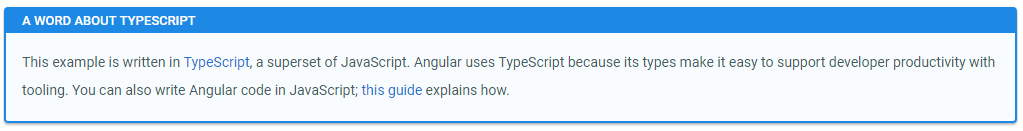
\includegraphics[width=\textwidth]{img/aboutTypescript.png}
        \end{center}
        \caption{Google sobre TypeScript}
    \end{figure}
    
    \subsection{¿Qué es un controlador?}\label{quuxe9-es-un-controlador}
    
    \begin{verbatim}
    @Component({
        selector: ‘my-app’,
        template: <h1>Hello {{name}}</h1>
    })
    \end{verbatim}
    
    Todos los componentes inician con el decorador \textcite{Component} que
    describe cómo se comporta el componente. Entre otras opciones, define
    como incluir el componente en una página HTML, mediante la propiedad
    selector; y como está estructurado visualmente mediante la propiedad
    template. En el ejemplo dado, si quisiéramos utilizar el componente en
    una página HTML se usaría el elemento
    \texttt{\textless{}my-app\textgreater{}}, y el componente se ve como la
    frase ``Hello \{\{name\}\}'' dentro de un elemento de de título 1.
    
    En un desarrollo de mayor tamaño en lugar de definir la plantilla HTML
    en el propio componente, se usará la propiedad \texttt{templateUrl} para
    definir dónde buscar la plantilla HTML. De igual forma, se separarían
    los códigos CSS mediante la propiedad \texttt{styleUrls}. Ejemplo:
    
    \begin{verbatim}
    @Component({
        selector: ‘my-app’,    
        templateUrl: 'nombre_del_archivo.html',
        styleUrls: ['nombre_del_archivo1.css', 'nombre_del_archivo2.css']
    })
    \end{verbatim}
    
    Siguiendo la trayectoria de AngularJs, precursor del actual Angular,
    conseguimos acceder a las propiedades del controlador mediante el uso de
    \{\{ nombre\_variable \}\}. En este caso accederíamos a la propiedad
    \texttt{name}.
    
    \begin{verbatim}
    export class AppComponent { name = ‘Angular’; }
    \end{verbatim}
    
    Define la clase del controlador. En el caso de ejemplo, el controlador
    solo tiene la propiedad name, que contiene la cadena de texto
    ``Angular''
    
    \section{Angular CLI}\label{angular-cli}
    
    \begin{figure}[H]
        \begin{center}
            
\includegraphics[scale=0.3]{img/angular-cli.png}
        \end{center}
        \caption{Logo de angular-cli}
    \end{figure}
    
    Angular CLI es una herramienta utilizada para inicializar aplicaciones
    Angular, desarrollar componentes y para tareas de mantenimiento
    asociadas a ello.
    
    \subsection{Instalacion:}\label{instalacion}
    
    \begin{verbatim}
    npm install -g @angular/cli
    \end{verbatim}
    
    \subsection{Comandos relevantes
    utilizados:}\label{comandos-relevantes-utilizados}
    
    \begin{itemize}
    \item
      \texttt{ng\ new\ {[}nombre{]}}
    
      Inicializa una nueva aplicación Angular con el nombre elegido.
    \item
      \texttt{ng\ serve}
    
      Transpila la aplicación y monta un servidor web.
    \item
      \texttt{ng\ generate\ class\ {[}nombre{]}}
    
      Genera una clase con el nombre escogido. Una clase es una construcción
      que permite crear tipos personalizados mediante la agrupación de
      variables de otras clases y comportamientos comunes.
    \item
      \texttt{ng\ generate\ component\ {[}nombre{]}}
    
      Genera un componente con el nombre escogido.
    \item
      \texttt{ng\ generate\ service\ {[}nombre{]}}
    
      Genera un servicio con el nombre escogido. Un servicio es una función,
      con sus propiedades y métodos que puede ser incluida, mediante
      inyección de dependencias, en los componentes. Gracias a esto, se
      pueden desarrollar funciones para tareas específicas, como es la
      comunicación con el servidor. Permite reutilizar las funciones de
      forma rápida entre componentes, así como acceder a variables
      compartidas entre ellos.
    \end{itemize}
    
    \section{Bootstrap 4}\label{bootstrap-4}
    
    \begin{figure}[H]
        \begin{center}
            
\includegraphics[scale=0.15]{img/bootstrap4.png}
        \end{center}
        \caption{Logo de Bootstrap 4}
    \end{figure}
    
    Bootstrap es un framework de HTML, CSS y JavaScript para el desarrollo
    de front-end. En su versión 4 incluye componentes de angular que
    utilizaremos en el presente proyecto.
    
    \subsection{Instalación}\label{instalaciuxf3n-3}
    
    \texttt{npm\ install\ bootstrap@4.0.0-alpha.6}
    
    \section{MariaDB}\label{mariadb}
    
    \begin{figure}[H]
        \begin{center}
            
\includegraphics[scale=0.75]{img/mariadb.png}
        \end{center}
        \caption{Logo de MariaDB}
    \end{figure}
    
    MariaDB es un sistema de gestión de bases de datos derivado de MySQL con
    licencia GPL (General Public License). Está desarrollado por Michael
    Widenius (fundador de MySQL) y la comunidad de desarrolladores de
    software libre. Surgío a partir de la compra de Sun Microsystems por
    parte de Oracle para asegurar la existencia de una versión de MySQL con
    licencia GPL.
    
    \subsection{Instalación}\label{instalaciuxf3n-4}
    
    \begin{verbatim}
    sudo apt-get install software-properties-common
    sudo apt-key adv --recv-keys --keyserver \
    keyserver.ubuntu.com 0xF1656F24C74CD1D8
    sudo add-apt-repository 'deb [arch=amd64] \
    http://tedeco.fi.upm.es/mirror/mariadb/repo/10.2/debian stretch main'
    sudo apt-get update
    sudo apt-get install mariadb-server
    \end{verbatim}
    
    \subsection{Ventajas de MariaDB frente
    MySQL}\label{ventajas-de-mariadb-frente-mysql}
    
    \begin{itemize}
    \item
      \textbf{Nuevos motores de almacenamiento más eficientes:}
    
      Aria y XtraDB vienen a reemplazar a MyISAM e InnoDB respectivamente.
      Cabe destacar el mayor rendimiento de Aria, cuando recibe consultas
      complejas y tiene que realizar tablas temporales, éstas se cachean en
      memoria en vez de escribirlas en disco.
    \item
      \textbf{Estadísticas para índices y tablas:}
    
      Esto puede ayudar para la optimización de la base de datos. Se añaden
      nuevas tablas de sistema para recoger esta información.
    \item
      \textbf{Mejoras en el rendimiento y la eficiencia con respecto a
      MySQL:}
    
      Un ejemplo de esto es la eliminación o mejora de algunas conversiones
      no necesarias respecto a los juegos de caracteres.
    \item
      \textbf{Software libre:}
    
      MariaDB está respaldada por la comunidad de software libre.
    \end{itemize}
    
    \subsection{Desventajas de MariaDB frente
    MySQL}\label{desventajas-de-mariadb-frente-mysql}
    
    \begin{itemize}
    \item
      \textbf{Coste migratorio:}
    
      En líneas generales, MySQL está más extendido, por lo que utilizar
      MariaDB suele acarrear un coste migratorio de los datos. Sin embargo,
      MariaDB asegura tener total compatibilidad. En este proyecto no nos
      afectará en absoluto.
    \end{itemize}
    
    \chapter{Desarrollo}\label{desarrollo}
    
    \section{Análisis}\label{anuxe1lisis}
    
    \subsection{Requisitos}\label{requisitos}
    
    \subsubsection{Requisitos funcionales}\label{requisitos-funcionales}
    
    \subsubsection{Requisitos no
    funcionales}\label{requisitos-no-funcionales}
    
    \subsubsection{Requisitos de
    información}\label{requisitos-de-informaciuxf3n}
    
    \subsection{Casos de uso}\label{casos-de-uso}
    
    \subsubsection{Diagrama de casos de uso}\label{diagrama-de-casos-de-uso}
    
    \subsubsection{Descripcion de los casos de
    uso}\label{descripcion-de-los-casos-de-uso}
    
    \subsection{Modelo de dominio}\label{modelo-de-dominio}
    
    \section{Diseño}\label{diseuxf1o}
    
    \subsection{Diseño de la base de
    datos}\label{diseuxf1o-de-la-base-de-datos}
    
    \subsection{Despliegue}\label{despliegue}
    
    \subsection{Arquitectura del sistema}\label{arquitectura-del-sistema}
    
    \subsubsection{Front-end}\label{front-end}
    
    \subsubsection{Back-end}\label{back-end}
    
    \subsection{Diagrama de clases}\label{diagrama-de-clases}
    
    \subsection{Diagramas de secuencia}\label{diagramas-de-secuencia}
    
    \chapter{Conclusiones}\label{conclusiones}
    
    Conclusiones
    
    \section{Trabajo futuro}\label{trabajo-futuro}
    
    Como mejorar la aplicacion
    
    \appendix
    
    \chapter{Manual de instalación}\label{manual-de-instalaciuxf3n}
    
    Test \autocite{rajwar_going_2012}.
    
    \chapter{Manual de usuario}\label{manual-de-usuario}
    
    \chapter{Contenido del CD-ROM}\label{contenido-del-cd-rom}
    
    \addcontentsline{toc}{chapter}{Bibliografía}
    
    \nocite{*} \printbibliography

    \cleardoublepage
    \addcontentsline{toc}{chapter}{Bibliografía}
    \printbibliography
    %\renewcommand\bibname{Referencias Web}

    %\begin{thebibliography}{X}
    %    \bibitem{ref1} \textit{Ejemplo}, \\
    %    \textsc{ejemplo.com}.
    %    \\Recuperado a tal fecha, \\de \href{http://ejemplo.com}
    %\end{thebibliography}
\end{document}
